\chapter{OPERACIONES PCE}

\section{Introducción} % {{{
%\cpnote{Porfa tambien esqueleto de la into}
%\esqueleto{ 
%\begin{itemize}
%\item Hablar que es importante estudiar problemas de muchas 
%partículas.
%\item Con la teoría de los canales cuánticos se pueden estudiar una 
%gran variedad de sistemas, siendo uno de ellos los de sistemas de qubits.
%\item Hablar qué son los qubits: sistemas cuánticos de dos niveles. 
%\cpnote{Creo que es un poco tarde para hablar de qubits. Ya mencionaste las matrices
%de Pauli, y sería buen momento antes, o de plano no decir nada.}
%\item Escribir sobre la estructura del capítulo.
%\end{itemize}
%}
%
%\esqueleto{
%\hrule\vspace{10pt}
%\h{Párrafos}
%\begin{itemize}
%\item Los sistemas cuánticos de dos niveles han sido y siguen 
%siendo de gran importancia teórica y práctica para la mecánica 
%cuántica y sus aplicaciones.
%\item La teoría de los canales cuánticos se puede utilizar para estudiar 
%la dinámica de un gran variedad de sistemas cuánticos abiertos, pero el objetivo
%de este proyecto está centrado en el estudio de los canales cuánticos de qubits.
%\item La estructura del capítulo.
%\end{itemize}
%}
%
%El tipo de operaciones que estudiamos en este trabajo son operaciones 
%que actúan sobre sistemas de qubits. Un qubit es un sistema cuántico 
%de dos niveles \janote{cita}, como una partícula de espín 1/2. Los 
%canales cuánticos de 1 qubit son especialmente útiles para ganar intuición
%sobre los canales cuánticos ya que los estados de 1 qubit se 
%pueden representar geométricamente en la esfera de Bloch \janote{cita}.
%Los estados de 1 qubit en la esfera de Bloch se pueden relacionar con 
%su matriz de densidad al escribir esta en la base de las matrices 
%de Pauli como 
%\begin{align}
%\rho=\frac{1}{2}\sum_{i=0}^3r_i\sigma_i
%\end{align}

\janote{La intro la dejo para cuando termine de escribir el capítulo.}

% }}}
\section{Operaciones PCE} % {{{
%\esqueleto{
%Dos o tres párrafos máximo hablando sobre las operaciones PCE 
%como operaciones proyectivas a la base de productos tensoriales de 
%las matrices de Pauli. Me gustaría poner un problema de motivación
%sólo para hacer más interesante la lectura a partir de acá y dejarle al
%lector algo con lo que pueda entender qué onda con las operaciones 
%PCE. Propongo lo siguiente: cadena de espines. Supongamos una 
%cadena de espines de $N$ sitios y decimos que nos interesa saber 
%si la matriz de densidad del $i$-ésimo espín puede proyectarse 
%al subespacio cuya base son $\sigma_x$ y $\sigma_y$ (lo que 
%quiero decir es que $(r_x,r_y,r_z)\to(r_x,r_y,0)$). Entonces hablo 
%de que hay que considerar que el $i$-ésimo espín puede estar 
%entrelazado con el resto de la cadena, sin embargo, basta con considerar
%que se encuentra entrelazado con cualquiera de sus vecinos y revisar 
%en qué se transforma la matriz de densidad de esos dos espines para 
%averiguar si es posible tal evolución física. Me gustaría poner unas 
%figuritas para hacer interesante esto. 
%}

%\esqueleto{La idea central de esta sección será: No todas las operaciones que 
%borran componentes de Pauli de la matriz de densidad de 1 qubit no 
%son canales cuánticos.}
%
%\esqueleto{Introducir los canales cuánticos de 1 qubit 
%de bit-flip y defasing como una motivación para definir qué es una 
%operación PCE. Figuritas para la interpretación geométrica y discutir 
%especialmente cómo actúan sobre las componentes de Pauli.}

En esta sección vamos a elaborar una discusión que conducirá a
la definición de una operación PCE y al planteamiento del problema
a tratar en esta tesis. 
Comenzaremos por introducir a los canales cuánticos  
\textit{bit-flip} y \textit{defasing} de 1 qubit. 
Ambos canales cuánticos son operaciones que mapean 
la esfera de Bloch a un elipsoide con eje mayor sobre los ejes $x$ y $z$, 
como se muestra en las Figs. \ref{fig:bit-flip} y \ref{fig:phase-flip}, 
respectivamente.
\begin{figure}
\centering
\begin{minipage}{.4\textwidth}
    \centering
    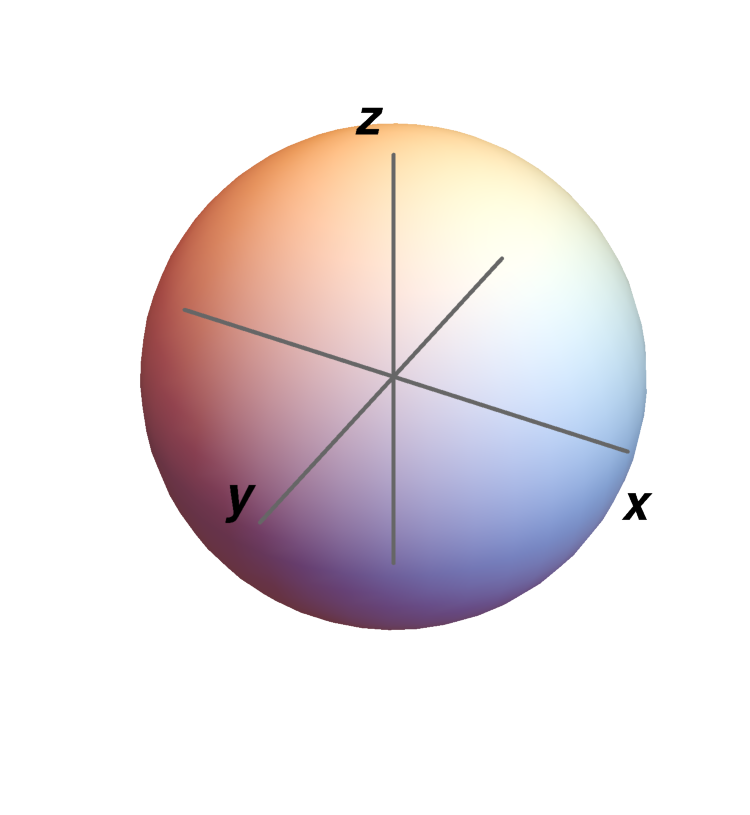
\includegraphics[width=3.8cm]{bloch-ball}
\end{minipage}
\LARGE{$\longmapsto$}
\begin{minipage}{0.4\textwidth}
    \centering
    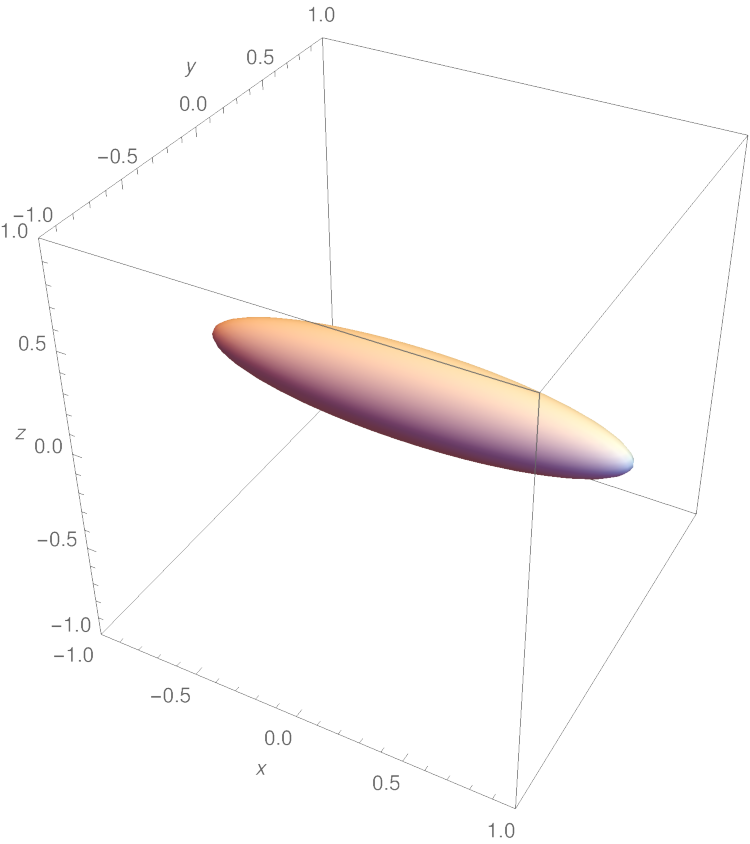
\includegraphics[width=3.8cm]{bit-flip}
\end{minipage}
\caption{
Efecto del canal de inversión de bit sobre la esfera de Bloch, para $p=0.3$.}
\label{fig:bit-flip}
\end{figure}
Para entender algebraicamente cómo actúan estos canales cuánticos 
recordemos que la matriz de densidad de 1 qubit se escribe en la 
base de matrices de Pauli como
\begin{align}\label{eq:rho-1qubit-ch2}
\rho=\frac{1}{2}\sum_{i=0}^3r_i\sigma_i,\hspace{2cm}r_0=1,
\end{align}
donde $r_1$, $r_2$ y $r_3$ especifican las coordenadas $\qty(x,y,z)$ 
del vector de Bloch. El canal \textit{bit-flip} transforma a las componentes 
de \eqref{eq:rho-1qubit-ch2} como~\cite{nielsen_chuang_2011}
\begin{align}\label{eq:bit-flip-transformation}
\qty(1,r_1,r_2,r_3)\longmapsto \qty(1,r_1,(1-2p)r_2,(1-2p)r_3),
\hspace{.5cm} 0\leq p\leq 1.
\end{align}
% \cpnote{Para $p=-1$ si es un canal cuantico? no, hay algo acá que está mal.}
% \janote{Me confundí, pero corregido}
Similarmente, el canal \textit{defasing} actúa sobre las mismas
componentes $r_i$ de \eqref{eq:rho-1qubit-ch2}
como~\cite{nielsen_chuang_2011}
\begin{align}\label{eq:defasing-transformation}
\qty(1,r_1,r_2,r_3)\longmapsto \qty(1,(1-2p)r_1,(1-2p)r_2,r_3),
\hspace{.5cm} 0\leq p\leq 1.
\end{align}
\begin{figure}
\centering
\begin{minipage}{.4\textwidth}
    \centering
    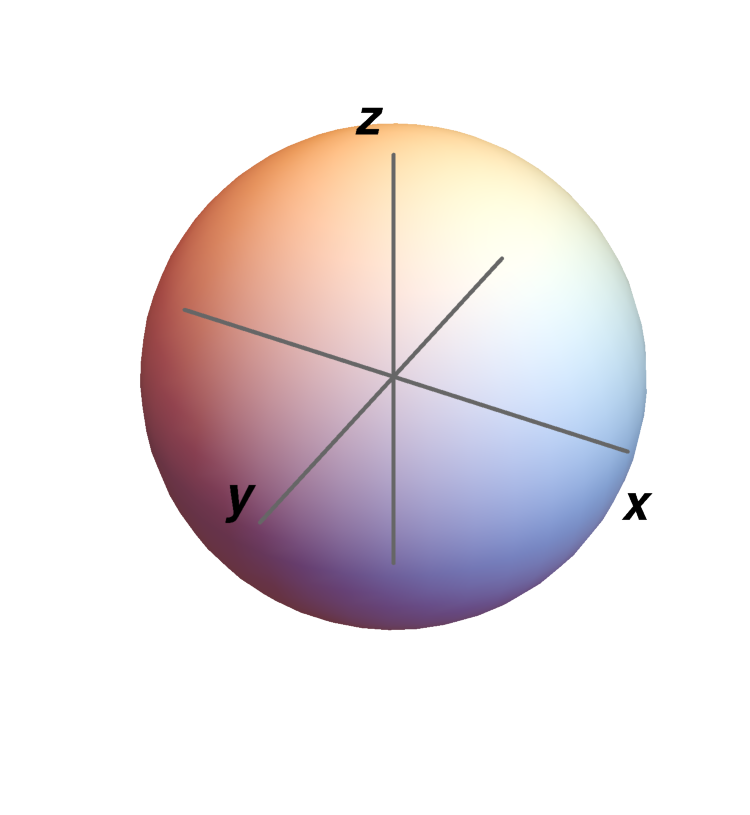
\includegraphics[width=4cm]{bloch-ball}
\end{minipage}
\LARGE{$\longmapsto$}
\begin{minipage}{0.4\textwidth}
    \centering
    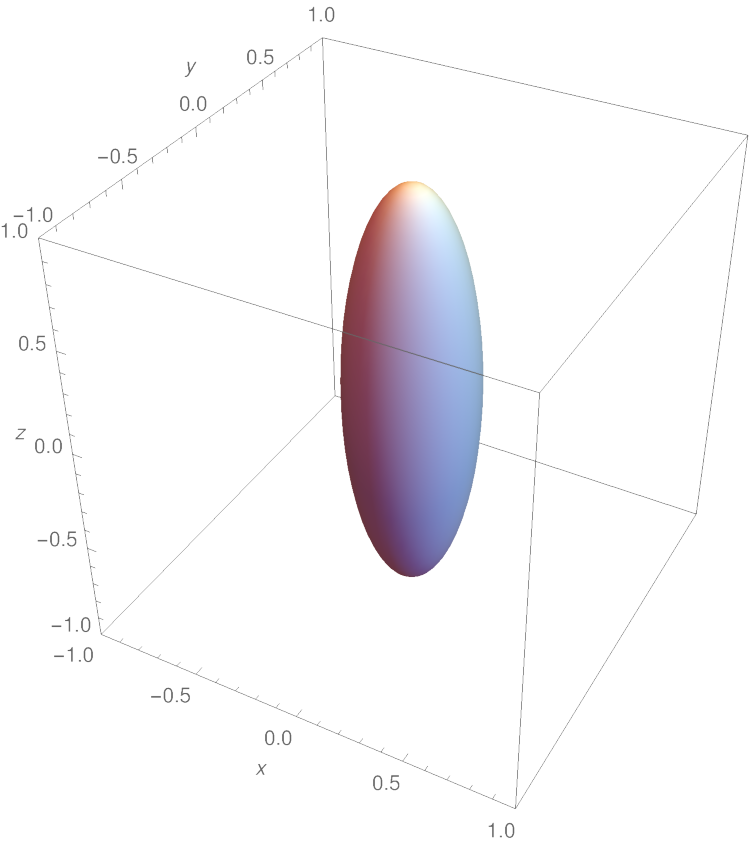
\includegraphics[width=4cm]{phase-flip}
\end{minipage}
\caption{
Acción geométrica del canal defasing de 1 qubit sobre la 
esfera de Bloch, para $p=0.3$.}
\label{fig:phase-flip}
\end{figure}
%\esqueleto{Mencionar los casos del bit-flip y defasing
%cuando la esfera de Bloch se mapea a una linea sobre los ejes $x$ y $y$,
%respectivamente. Nada nuevo, evidentemente son canales porque son 
%casos particulares de otros que son canales. Introducir el punto de vista
%de esos canales como operaciones que borran componentes.}
Vamos a detenernos a analizar qué ocurre cuando $p=1/2$. 
En este caso, \eqref{eq:bit-flip-transformation} y
\eqref{eq:defasing-transformation} se escriben
\begin{align}\label{eq:bit-flip_p=0.5}
\qty(1,r_1,r_2,r_3)&\longmapsto \qty(1,r_1,0,0),\\
\qty(1,r_1,r_2,r_3)&\longmapsto \qty(1,0,0,r_3).\label{eq:defasing_p=0.5}
\end{align}
Es decir que, el \textit{bit-flip} y \textit{defasing} cuando $p=1/2$
son operaciones que mapean la esfera de Bloch a una línea sobre 
el eje mayor de los elipsoides en las Figs. \ref{fig:bit-flip} y \ref{fig:phase-flip}.
Va a ser útil que interpretemos a estos canales cuánticos 
como operaciones que `borran' dos de las proyecciones
$r_i$  de la matriz de densidad de 1 qubit sobre
las matrices de Pauli y que dejan al resto de componentes $r_j$ invariantes.
% \cpnote{La redacción está como 
% chistosa. Por cierto lo de arrancar diciendo ``probara ser \ldots'' suena a 
% anglisismo. Porfa considera cambiar eso. } 
% \janote{Listo}

%\esqueleto{Conducir al lector a preguntarse: `bueno, entonces deplano
%que puedo borrar cualquier cantidad de componentes de Pauli, ¿no? ¡¿NO?!', 
%pero nel. Recordar que vimos en el capítulo anterior la operación que 
%mapea la esfera de Bloch a un disco sobre el plano $x$-$y$ y no es 
%un canal cuántico... porque no es CP. Es decir, la condición de completa 
%positividad es la que impide que las operaciones que borran componentes 
%de Pauli de 1 qubit sean trivialmente canales cuánticos. Siempre será bueno
%que dedique al menos una frase a recordar la implicación física de la CP: 
%existe por lo menos un estado entrelazado en el espacio de 2 qubits 
%que se mapea a un no estado.}

Las operaciones 	que se describen en \eqref{eq:bit-flip_p=0.5}
y \eqref{eq:defasing_p=0.5} sugieren preguntarse si todas las
operaciones que borran cualesquiera de las componentes $r_i$ 
de la matriz de densidad de 1 qubit 
en \eqref{eq:rho-1qubit-ch2} son canales cuánticos.
La pregunta es relevante porque la respuesta es
que no\cpnote{Se me hace una justificación mala. Quiza podemos quitar
esa frase}. En el capítulo anterior, en la sección 
\ref{sec:qtm-channels}, elaboramos el ejemplo de la operación $\E_z$
que borra la componente $r_3$ y demostramos que no es un canal 
cuántico porque no es una operación completamente positiva. 
Vimos que no satisfacer esta condición implica que la operación 
$\E_z\ot\1$, que actúa sobre una matriz de densidad de 2 qubits,
no transforma a la matriz 
de densidad del estado máximamente entrelazado en otra 
matriz de densidad.
Es decir, la operación $\E_z$ es un ejemplo de una 
operación de 1 qubit que borra un subconjunto de las componentes $r_i$ de 
la matriz de densidad \eqref{eq:rho-1qubit-ch2} y que no es canal cuántico.

%\esqueleto{Motivar a pensar que si la CP ya impide que algunas 
%operaciones que borran componentes de Pauli de 1 qubit no sean
%canales cuánticos entonces ¿qué ocurrirá en sistemas de más qubits 
%que ya aparecen correlaciones cuánticas? (porque en el caso de 1 qubit 
%la regla de $2^k$ es necesaria y suficiente, para más qubits también 
%va a importar cuáles componentes se borran y en este punto debería 
%ser una pregunta importante para quien no sepa la respuesta)}

La restricción que impone la completa positividad a un canal cuántico 
vuelve interesante estudiar a los canales cuánticos que borran las componentes 
de la matriz de densidad de un sistema de qubits en la base de matrices 
de Pauli. Revisemos el problema de 2 qubits. La matriz de densidad
se escribe
\begin{align}\label{eq:rho_2qubits_cap2}
\rho = \frac{1}{4}\sum_{i,j=0}^3r_{ij}\sigma_i\ot\sigma_j, 
\hspace{2cm} r_{0,0}=1.
\end{align}
Hay 15 componentes $r_{ij}$ que se podrían borrar o dejar invariantes. 
Por consiguiente, hay $32,768$ $(2^{15})$ operaciones distintas que borran las 
componentes de la matriz de densidad \eqref{eq:rho_2qubits_cap2} de 2 qubits. 
El número de operaciones de este tipo crece de manera \cpnote{de hecho doblemente
exponencial} exponencial 
como $2^{4^n-1}$, con $n$ el número de qubits. Sin embargo, no es 
sólo el crecimiento exponencial en el número de operaciones de este tipo
lo que hace interesante al problema, sino también el hecho de que en 
sistemas de más de 1 qubit aparecen correlaciones cuánticas entre 
las particiones del sistema. Por consiguiente, no es trivial inferir cuáles son los 
canales cuánticos que borran las componentes $r_{ij}$ de 
\eqref{eq:rho_2qubits_cap2} a partir de los canales cuánticos 
de 1 qubit que borran las componentes $r_i$ de \eqref{eq:rho-1qubit-ch2}.

%\esqueleto{Ya, no más rodeos y finiquitar con la expresión de $\rho$ para 
%$n$ qubits en la base de Pauli y definir formalmente una operación PCE.}

Sin más, introducimos ahora la definición de una operación PCE de 
$n$ qubits. La matriz de densidad de un sistema de $n$ qubits, en la base de
productos tensoriales de las matrices de Pauli, se escribe como
\begin{align}\label{eq:rho_n_qubits}
\rho=\frac{1}{2^n}\sum_{j_1,\ldots,j_n=0}^3
r_{j_1,\ldots,j_n}\sigma_{j_1}\ot\ldots\ot\sigma_{j_n},
\hspace{2cm} r_{0,\ldots,0}=1.
\end{align}
Vamos a llamar ``componentes de Pauli'' a los coeficientes $r_{j_1,\ldots,j_n}$
de \eqref{eq:rho_n_qubits}. Las componentes de Pauli son las proyecciones
de la matriz de densidad de un sistema de $n$ qubits sobre los elementos
de la base de productos tensoriales de las matrices de Pauli.
Llamamos una operación que borra las componentes de Pauli, 
operación PCE por sus siglas en inglés (\textit{Pauli
component erasing}), a una operación lineal que actúa sobre una 
matriz de densidad de la forma \eqref{eq:rho_n_qubits} y 
que transforma a las componentes de Pauli como
\begin{align}\label{eq:PCE_definition}
r_{j_1,\ldots,r_n}\longmapsto \tau_{j_1,\ldots,r_n}r_{j_1,\ldots,r_n},
\hspace{1cm} \tau_{j_1,\ldots,r_n} = 0,1,
\hspace{1cm} \tau_{0,\ldots,0}=1.
\end{align}
En otras palabras, una operación PCE es una operación lineal que actúa sobre la
matriz de densidad de $n$ qubits y que borra a algunas de las componentes de
Pauli y deja invariantes al resto.
A las operaciones PCE que satisfacen 
la condición de completa positividad y son, por ende, canales cuánticos,
les llamaremos ``canales cuánticos PCE'' o sólamente ``canales PCE''.

De manera muy puntual, podemos formular el problema para 
este trabajo con la siguiente pregunta: ¿qué características tienen 
en común y qué condiciones satisfacen todos los canales PCE 
de sistemas de 2 y 3 qubits? Dicho de otro modo, 
nuestro objetivo es investigar qué hace de diferente la condición de 
completa positividad a los canales PCE del conjunto de todas las 
operaciones PCE de 2 y 3 qubits.
En las siguientes secciones presentaremos el estudio analítico del 
caso de 1 qubit y el método numérico que diseñamos 
para estudiar sistemas de 2 y 3 qubits. 


% }}}
\section{1 qubit} % {{{
%\esqueleto{
%Idea central de esta sección: encontrar todos los canales cuánticos PCE 
%de 1 qubit.}
%
%\esqueleto{
%Para resolver el problema lo que haremos será encontrar los eigenvalores 
%de la matriz de Choi del superoperador y así encontrar las condiciones 
%que debe satisfacer una operación PCE de 1 qubit para ser un canal cuántico
%en términos de las $\tau_i$. 
%Escribir al superoperador, en su forma diagonal con las $\tau_i$, 
%que actúa sobre la matriz de densidad de 1 qubit escrita en la base de Pauli. 
%}

El problema de los canales PCE de 1 qubit puede ser resuelto analíticamente
y vamos a discutir cómo en esta sección. 
Vamos a presentar nuestro procedimiento para evaluar analíticamente 
la completa positividad de las operaciones PCE de 1 qubit.
De acuerdo con el teorema \ref{thm:choi-CP}, podemos determinar si
una operación es completamente positiva evaluando que su 
matriz de Choi sea una matriz positiva semidefinida.
Por lo tanto, vamos a buscar diagonalizar la matriz de Choi en 
función de los elementos $\tau_i$ de la operación PCE. Así, evaluar
que todos los eigenvalores sean no negativos para 
cada uno de los arreglos de 1's y 0's de las $\tau_i$ que 
caracteriza a las operaciones PCE de 1 qubit 

Enunciamos ahora nuestro algoritmo para evaluar la completa 
positividad de una operación PCE de 1 qubit. 
\begin{enumerate}
	\item Escribir al superoperador de una operación PCE en 
	la base de matrices de Pauli $\sigma_i$ (con $\sigma_0=\1$), 
	base en la cual es diagonal. En general, en la base de Pauli
	el superoperador de una 	operación PCE de 1 qubit se escribe
	\begin{align} \label{eq:supOp_PCE_1q}
		\Phi=\mqty(\dmat[0]{1,\tau_1,\tau_2,\tau_3}).
	\end{align}
	\item Hacer un cambio de base al superoperador \eqref{eq:supOp_PCE_1q}, 
	de la base de matrices de Pauli a la base computacional, vía $P \Phi P^{-1}$, 
	con
	\begin{align}
		P = \mqty(1&0&0&1\\ 0&1&-i&0\\ 0&1&i&0 \\ 1&0&0&-1).
		%	\mqty(\dmat[0]{1,\tau_1,\tau_2,\tau_3})
		%	\mqty(
		% 	\frac{1}{2} & 0 & 0 & \frac{1}{2} \\
		% 	0 & \frac{1}{2} & \frac{1}{2} & 0 \\
		% 	0 & \frac{i}{2} & -\frac{i}{2} & 0 \\
		% 	\frac{1}{2} & 0 & 0 & -\frac{1}{2} \\
		%	)
		%	=
		%	\mqty(
		%	\frac{\tau _3}{2}+\frac{1}{2} & 0 & 0 & \frac{1}{2}-\frac{\tau _3}{2} \\
		% 	0 & \frac{\tau _1}{2}+\frac{\tau _2}{2} & \frac{\tau _1}{2}-\frac{\tau _2}{2} & 0 \\
		% 	0 & \frac{\tau _1}{2}-\frac{\tau _2}{2} & \frac{\tau _1}{2}+\frac{\tau _2}{2} & 0 \\
		% 	\frac{1}{2}-\frac{\tau _3}{2} & 0 & 0 & \frac{\tau _3}{2}+\frac{1}{2} \\
		%	)
	\end{align}
	Notemos que la matriz de cambio de base $P$ es una matriz 
	que se construye yuxtaponiendo las matrices de Pauli 
	vectorizadas $\vec{\sigma}_i$, 
	siguiendo la vectorización de una matriz como se definió en 
	\eqref{eq:matrix-to-vector}.
	\item Aplicar la transformación de \textit{reshuffle} a $P\Phi P^{-1}$,  
	según \eqref{eq:ChoiMatrix-via-reshuffle}, para 
	determinar la matriz de Choi de la operación PCE,
	\begin{align}\label{eq:choi_1q}
		\qty(P \Phi P^{-1})^R=
		\frac{1}{2}\mqty(
		\tau _3+1 & 0 & 0 & \tau _1+\tau _2 \\
		0 & 1-\tau _3 & \tau _1-\tau _2 & 0 \\
		0 & \tau _1-\tau _2 & 1-\tau _3 & 0 \\
		\tau _1+\tau _2 & 0 & 0 & \tau _3+1 
		).
	\end{align}
	\item Por último, para evaluar si la matriz de Choi es positiva semidefinida, 
	calcular los eigenvalores $\lambda_i$ de \eqref{eq:choi_1q} y revisar que 
	todos sean 	iguales o mayores a cero,
	\begin{subequations}\label{eq:eigv_1qubit_PCE}
		\begin{align}
			\lambda_0=\frac{1}{2}& \left(1+\tau _1+\tau _2+\tau _3\right)\geq0, \\
			\lambda_1=\frac{1}{2}& \qty(1+\tau _1-\tau _2-\tau _3)\geq0, \\
			\lambda_2=\frac{1}{2}& \left(1-\tau _1+\tau _2-\tau _3\right)\geq0, \\
			\lambda_3=\frac{1}{2}& \left(1-\tau _1-\tau _2+\tau _3\right)\geq0.
		\end{align}
	\end{subequations}
	Debemos remarcar que en ninguno de los pasos hemos utilizado el hecho de que
	para una operación PCE las componentes $\tau_i$ sean iguales a cero o uno,
	como está definido en \eqref{eq:PCE_definition}. Por lo tanto, las 
	desigualdades en \eqref{eq:eigv_1qubit_PCE} caracterizan la completa 
	positividad de una operación lineal de 1 qubit que actúa sobre las
	componentes de Pauli como $r_i\longmapsto \tau_ir_i$, donde $\tau_i$
	puede tomar cualquier valor. Considerando eso, 
	las desigualdades en \eqref{eq:eigv_1qubit_PCE} coinciden con las 
	que presentan 	Bengtsson y Życzkoski
	 \cite[pág. 292]{bengtsson_zyczkowski_2017}.
\end{enumerate}

\begin{table}[] 
\centering
\begin{tabular}{|l|l|l|l|}
\hline
           & $\tau_1$ & $\tau_2$ & $\tau_3$ \\ \hline
\textbf{1} & 1        & 1        & 1        \\ \hline
\textbf{2} & 1        & 1        & 0        \\ \hline
\textbf{3} & 1        & 0        & 1        \\ \hline
\textbf{4} & 0        & 1        & 1        \\ \hline
\textbf{5} & 1        & 0        & 0        \\ \hline
\textbf{6} & 0        & 1        & 0        \\ \hline
\textbf{7} & 0        & 0        & 1        \\ \hline
\textbf{8} & 0        & 0        & 0        \\ \hline
\end{tabular}
\caption{Combinaciones de $\tau_i$ de todas las operaciones PCE de 1 qubit. 
\cpnote{Creo que esta tabla podría ser mas completa. Podrías incluir la
información de cuales son validas y quizá también un indicador del número de componentes
que permanecen invariantes. }}
\label{tab:1qubit_PCE}
\end{table}

Previo a determinar los canales PCE de 1 qubit enunciamos en la Tabla
\ref{tab:1qubit_PCE} todos los arreglos de 1's y 0's de las 
componentes $\tau_i$ de cada una de las 8 operaciones PCE de 1 qubit. 
Es útil que discutamos la acción geométrica sobre la esfera de Bloch de 
cada una de las operaciones PCE de 1 qubit en la Tabla \ref{tab:1qubit_PCE}.
El arreglo 1 es la operación identidad. Los arreglos 2-4 son operaciones
que mapean la esfera de Bloch a un disco que es perpendicular 
a cada uno de los ejes cartesianos. Los arreglos 
5-7 son operaciones que mapean la esfera de Bloch a una línea sobre cada
uno de los ejes cartesianos. Y, por último, el arreglo 8 es la operación 
que mapea la esfera de Bloch a un punto sobre el origen de coordenadas. 

Al evaluar la completa positividad de cada operación PCE en la Tabla
\ref{tab:1qubit_PCE}, comprobando que cada arreglo $\tau_i$ 
satisfaga las desigualdades en \eqref{eq:eigv_1qubit_PCE},
encontramos que 5 de las 8 operaciones PCE de 1 qubit
son canales cuánticos. Las matrices de Choi de las operaciones PCE 
2, 3 y 4 de la Tabla \ref{tab:1qubit_PCE} tienen un eigenvalor que es negativo. 
Por ejemplo, el eigenvalor $\lambda_3$ de la operación PCE 2 
es igual $-1/2$. Es decir que, entonces, son canales PCE de 1 qubit 
sólo la operación identidad, las operaciones que 
mapean la esfera de Bloch a una línea sobre los ejes cartesianos y la 
operación que mapea la esfera de Bloch al origen de coordenadas.

%
%\esqueleto{
%Aplicar el reshuffle para encontrar la matriz de Choi y calcular después 
%sus eigenvalores.
%}
%
%\esqueleto{
%Enunciar las desigualdades que deben satisfacer las $\tau_i$ para que 
%la operación sea un canal cuántico. Hacer referencia al resultado del
%Geometry of Quantum States en el que también llegan a esas desigualdades
%(tienen un nombre). Esto para hacerlo ver como un check de que no 
%estamos hablando paja aquí.
%}
%
%\esqueleto{
%Escribir las 8 operaciones PCE de 1 qubit y discutir sobre las operaciones 
%que sí satisfacen las desigualdades para ser canales cuánticos y las que no.
%Discutir que no hay nada fundalmente diferente entre las 3 operaciones
%que mapean la esfera de Bloch a una línea, igual que las 3 que mapean 
%la esfera de Bloch a un disco. Esto implica que hay una equivalencia
%entre esas operaciones. 
%Y fin. En conclusión, son canales cuánticos PCE solo los que dejan igual 
%la esfera de Bloch, mapean la esfera de Bloch a una línea o al origen de
%coordenadas. 
%}

%\esqueleto{
%Resumen de los resultados de 1 qubit. Para seguir un orden lógico
%en este capítulo voy a hablar de los resultados de 1 qubit con el 
%problema resuelto analíticamente (está medio desordenado 
%si hablo por acá del método numérico y luego lo vuelvo a hacer 
%en la sección 2.5), a partir de las desigualdades
%de los eigenvalores (el polihedro?).
%}

%\cpnote{Está bien. Acá antes de escribir quiero un esqueleto más detallado. Lo mismo para las siguientes secciones, 2.3, 2.4 y 2.5}
%
%\esqueleto{ 
%\begin{itemize}
%\item Escribir a $\rho$ de 1 qubit en la base de las matrices de Pauli.
%\item Enunciar las 8 operaciones PCE de 1 qubit.
%\item Desarrollar cómo verificar analíticamente si las operaciones PCE 
%de 1 qubit son CP. Es decir, partir de 
%\begin{align*}
%\left(
%\begin{array}{cccc}
% 1 & 0 & 0 & 0 \\
% 0 & \tau _1 & 0 & 0 \\
% 0 & 0 & \tau _2 & 0 \\
% 0 & 0 & 0 & \tau _3 \\
%\end{array}
%\right)
%\end{align*}
%calcular el estado de Jamiolkowsky y verificar si es positivo. Con esto llegaré 
%a las desigualdades.
%\item Con las desigualdades revisar los casos para sacar los 5 canales 
%cuánticos PCE.
%\item Discutir que las operaciones PCE que borran 1 y 2 componentes 
%de Bloch (3 operaciones cada una) son equivalentes bajo permutación 
%de los elementos de la base de las matrices de Pauli. Esto me servirá 
%para retomarlo después con el argumento de que los canales cuánticos
%son equivalentes con permutaciones locales de los elementos de la base 
%y de los swaps de partículas. 
%\item Final: resumencillo de que hay 8 operaciones PCE, pero sólo 5 son 
%CP (y por tanto evoluciones físicas).
%\end{itemize}
%}

%\esqueleto{
%\hrule \vspace{10pt}
%\h{Párrafos}
%\begin{itemize}
%\item Las operaciones PCE de 1 qubit transforman a las componentes
%de Bloch $r_i$ como $r_i\to \tau_ir_i$, donde $\tau_i=0,1$.
%\item Hay 8 operaciones PCE posibles para 1 qubit.
%\item La completa positividad está determinada por un set de 4 desigualdades.
%\item Las tres operaciones PCE que borran 1 y 2 componentes del vector 
%de Bloch, respectivamente, son equivalente bajo permutación de las 
%matrices de Pauli $\sigma_i$ en la base 
%$\{\sigma_0,\sigma_1,\sigma_2,\sigma_3\}$.
%\item Cinco de las ocho operaciones PCE son completamente positivas y,
%por consiguiente, canales cuánticos.
%\end{itemize}
%}
% }}}
\section{El problema de $\mathbf{n}$ \cpnote{No quedó bien la $n$, porfa corrige} qubits} % {{{ 
\label{sec:n_qubits_problem}

%\esqueleto{
%La idea central de esta sección es que para el problema de n qubits la 
%solucion son los mismos pasos que para el problema de 1 qubit, pero
%la diagonalización exacta de la matriz de Choi no es así nomás. Por lo tanto, 
%hay que recurrir a otros métodos mientras no tengamos la diagonalización 
%para investigar sistemas de más de 1 qubit.\newline
%}
%En principio, podríamos buscar extender el algoritmo que describimos 
%para evaluar la completa positividad de las operaciones PCE de 1 qubit
%para sistemas de $n$ qubits. No obstante, la diagonalización de la 
%matriz de Choi 
%La diagonalización exacta de la matriz de Choi de una operación 
%PCE de $n$ qubits es un problema no trivial que nos obligó a
%implementar un método numérico para buscar los canales PCE 
%de 2 y 3 qubits.
%
%\esqueleto{
%Repetir el procedimiento de la sección anterior: (1) escribir al 
%superoperador en la base que es diagonal, (2) reshuffle, pero al llegar al
%paso (3), la diagonalización, discutir que el problema de que la
%diagonalización exacta es un problema difícil y para este trabajo 
%preferimos explorar una solución numérica.\newline
%}

El algoritmo  para evaluar la completa positividad de las operaciones PCE de 1
qubit, que discutimos en la sección anterior, se puede generalizar para $n$
qubits y es 
el tema que discutiremos en esta sección. A diferencia 
del problema de 1 qubit, en el problema de las operaciones PCE de $n$ qubits
la diagonalización exacta de la matriz de Choi es un problema no trivial. 
Por esa razón, decidimos explorar una alternativa para buscar 
los canales PCE de 2 y 3 qubits.

A continuación, discutimos la generalización de nuestro algoritmo 
para evaluar la completa positividad de una operación PCE de $n$ qubits.  
\cpnote{Sugiero hacer una lista con los pasos. Es mas facil de leer}
(1) Se escribe al superoperador $\Phi$
de una operación PCE, en la base de productos 
tensoriales de las matrices de Pauli, 
\begin{align}
\Phi=
\mqty(1&0&0&\hdots&0\\ 0&\tau_{0,\ldots,0,1}&0&\hdots&0\\
0&0&\tau_{0,\ldots,0,2}&\hdots&0\\
\vdots&\vdots&\vdots&\ddots&\vdots\\
0&0&0&\hdots&\tau_{1,\ldots,1,1}),
\end{align}
con $\tau_{j_1,\ldots,j_n}$ las componentes de la operación PCE como 
se definió en \eqref{eq:PCE_definition}.
(2)~Se hace el cambio de base $P\Phi P^{-1}$ para 
escribir al superoperador $\Phi$ en la base computacional. 
$P$ es la matriz de cambio de base y se construye yuxtaponiendo 
las matrices 
vectorizadas de los productos tensoriales de las matrices de Pauli\cpnote{Puedes
ser mucho mas explicito y dar la formula con productos tensoriales, o quizá
ya la diste antes y la puedes referenciar}.
(3) Se determina la matriz de Choi según $D_{\Phi}=\qty(P\Phi P^{-1})^R$, 
aplicando el \textit{reshuffle} a la matriz $P\Phi P^{-1}$. 
(4) Por último, se calculan los eigenvalores de $D_{\Phi}$ y si
todos son positivos o cero, entonces $\Phi$ es un canal cuántico\cpnote{Ojo, 
el algoritmo es para evaluar la completa positividad por lo que este ultimo 
punto como qe no es parte del algoritmo sino una nota adicional}. 
Es este último paso el que supone una dificultad en la generalización 
de nuestro algoritmo.
La ecuación $\det\qty(D_{\Phi}-\lambda \1)=0$, que hay que resolver
para determinar los eigenvalores $\lambda_{j_1\ldots,j_n}$,
es una ecuación de grado $4^n$. Esto hace que la diagonalización 
exacta de la matriz de Choi $D_{\Phi}$, de una operación PCE de $n$ 
qubits, sea un problema algebraicamente complicado. 
En vista de esta dificultad, decidimos utilizar herramientas computacionales
para evaluar numéricamente la positividad de la matriz de Choi $D_{\Phi}$ 
de las operaciones PCE de 2 y 3 qubits y así determinar los canales cuánticos.  

% \vfill

% }}}
\section{Solución numérica}\label{sec:ch2_solucionNumerica} % {{{
%\esqueleto{
%La idea central de esta sección es describir el método numérico para 
%resolver 2 y 3 qubits (hay que discutir qué y cómo vamos a escribir lo 
%de 3 qubits porque el primer método numérico de fuerza bruta no puede 
%resolver completo 3 qubits).\newline
%}

Propusimos evaluar numéricamente la completa positividad de las 
operaciones PCE de 2 y 3 qubits para encontrar los  
canales cuánticos, y en esta sección vamos a describir las herramientas
computacionales que desarrollamos y la implementación 
del método numérico. Para esto, diseñamos rutinas que 
implementan el algoritmo descrito en la sección anterior.
El método numérico consiste en generar todas \cpnote{Según entendí de hecho 
no generamos todas. Afinar las palabras}
las operaciones PCE de 2 y 3 qubits, evaluar si son completamente positivas
y, dependiendo de ello, agrupar a los canales cuánticos PCE para luego 
analizar sus características en el próximo capítulo.

Las rutinas se programaron en el lenguaje de Wolfram\cpnote{No se que 
tan preciso es eso. Mas bien se programan con Mathematica, no?}.
Con estas rutinas, se pueden generar
todos los diferentes arreglos de 1's y 0's, de los elementos de 
transformación $\taus$,
que definen a cada operación PCE y evaluar, una por una, si
es completamente positiva.
A continuación, describimos brevemente cada una de las rutinas que diseñamos.
\begin{enumerate}
	\item \textbf{Pauli[\texttt{Indices}]}: calcula el producto tensorial 
	de las matrices 	de Pauli $\sigma_i$ con índices $i$ en el 
	arreglo 1-D \texttt{Indices}\janote{Está bien este tipo de letra 
	para cosas de 'código'?}\cpnote{si, es el tipo de letrta que se usa
para codigo, pero entonces usala consistentemente para todo el codigo, 
incluyendo los nombres de las rutinas y las variables}.
	\item \textbf{PCEsTauConfigurations[\textit{n}]}: devuelve todos
	los arreglos de 1's y 0's de los elementos $\taus$
	de todas las operaciones PCE de $n$ qubits.
	\item \textbf{PCEsTauConfigurations[\textit{n,k}]}: devuelve todos 
	los arreglos de 1's y 0's de los elementos $\taus$
	de todas las operaciones PCE de $n$ qubits que dejan $k$ 
	componentes de Pauli invariantes.
	\item \textbf{PCESuperoperator[$\tau$]}: calcula el superoperador en 
	la base computacional de una operación PCE, dados los elementos
	$\tau_{j_1,\ldots,j_n}$	en el arreglo 1-D $\tau$.	
	\item \textbf{Reshuffle[\textit{m}]}: aplica la transformación de 
	\textit{reshuffle} a la matriz \textit{m} de dimensión $d^2\times d^2$.
	Esta función implementa la definición \eqref{eq:Reshuffle_4-indices}.
	\item \textbf{PositivityTest[\textit{m}]}: revisa si la matriz \textit{m}
	es positiva semidefinida. Devuelve el valor \textit{True} si lo es y 
	\textit{False} en caso contrario. 
	\item \textbf{PCEFigures[$\boldsymbol{\tau}$]}: grafica la representación 
	geométrica de los elementos $\tau_{j_1,\ldots,j_n}$ en el arreglo 
	1-D $\tau$ de una operación PCE de 1, 2 o 3 qubits. 
	\item \textbf{TausOfPCEQuantumChannels[$\boldsymbol{n}$]}: 
	devuelve todos los arreglos de 1's y 0's de los elementos 
	$\taus$ de los canales 	cuánticos PCE de $n$ qubits.
	\item \textbf{TausOfPCEQuantumChannels[$\boldsymbol{n,k}$]}: 
	devuelve todos los arreglos de 1's y 0's de los elementos 
	$\taus$ de los canales cuánticos PCE de $n$ qubits que dejan $k$
	componentes de Pauli invariantes.
	\item \textbf{TausOfPCEQuantumChannels[$\boldsymbol{n,k_{min},
	k_{max}}$]}: 
	devuelve todos los arreglos de 1's y 0's de los elementos 
	$\taus$ de los canales cuánticos PCE de $n$ qubits que dejan desde 
	$k_{min}$ hasta $k_{max}$	componentes de Pauli invariantes.
	\item \textbf{NumberOfPCEOperations[$\boldsymbol{n}$]}: calcula 
	el número total de operaciones PCE de $n$ qubits. 
	\item \textbf{NumberOfPCEOperations[$\boldsymbol{n,k}$]}: calcula 
	el número total de operaciones PCE de $n$ qubits que dejan $k$
	componentes de Pauli invariantes. 	
\end{enumerate}
Todas estas rutinas las agrupamos en un paquete de Mathematica
que se puede encontrar en un repositorio de libre acceso en 
GitHub\footnote{Se puede encontrar en 
\href{https://github.com/deleonja/projective_maps}
{https://github.com/deleonja/projective\_maps} bajo 
el nombre "pce.m".}. Específicamente, las rutinas 
\textbf{Pauli}, \textbf{PCESuperoperator}, \textbf{Reshuffle} y 
\textbf{PositivityTest} fueron diseñadas para reproducir los pasos 
del algoritmo para evaluar la completa positividad de una operación 
PCE de $n$ qubits de la sección \ref{sec:n_qubits_problem}.
El algoritmo completo fue implementado en la rutina 
\textbf{TausOfPCEQuantumChannels}\cpnote{todas estas tambien con el tipo de letra 
apropiado}. Debe notarse en la definición 
\eqref{eq:PCE_definition}, de una operación PCE, que la lista de
1's y 0's de los elementos de transformación $\taus$ caracteriza 
por completo a la operación. Por ejemplo, la operación PCE de 1 qubit 
que mapea la esfera de Bloch a un punto en el origen
está completamente determinada por 
los elementos $\tau_i$ $\{1,0,0,0\}$; esta lista de 
1's y 0's es suficiente para encontrar al correspondiente superoperador.
Dicho esto, describimos con detalle la rutina 
\textbf{TausOfPCEQuantumChannels} a continuación.
%\esqueleto{
%Para implementar el método numérico utilizamos el lenguaje de Wolfram 
%Alpha. El algoritmo implementado fue: 
%\begin{enumerate}
%\item Escribir una posible configuración de $\vec{\tau}$ de 1's y 0's.
%\item Aplicar la transformación de reshuffle.
%\item Calcular los eigenvalores de la matriz de Choi. 
%\item Revisar que todos los eigenvalores sean no negativos.
%\end{enumerate}
%}

%\noindent\rule{\textwidth}{1mm}
%\textbf{Canales cuánticos PCE.} Algoritmo para determinar si una 
%operación PCE es completamente positiva. \textbf{Entrada:} Arreglo 
%1-D $\tau$ con los elementos $\tau_{j_1,\ldots,j_n}$ de la operación PCE. 
%\textbf{Salida:} Valor booleano ``\textit{True}'' si la operación 
%PCE es completamente positiva y ``\textit{False}'' en caso contrario. 
%\textbf{Utiliza:} PCESuperoperator, Reshuffle y PositivityTest.
%\begin{enumerate}
%	\item Calcular el superoperador $\Phi$, en la base computacional, 
%	de la operación PCE con PCESuperoperator[$\tau$].
%	\item Calcular la matriz de Choi $D_{\Phi}$ de la operación PCE 
%	aplicando la función Reshuffle[] a la matriz del paso 1.
%	\item Calcular que la matriz del paso 2 sea positiva semidefinida 
%	con PositivityTest[].
%\end{enumerate}
%
%\noindent\rule{\textwidth}{1mm}

\noindent\rule{\textwidth}{1mm}
\textbf{TausOfPCEQuantumChannels.} Rutina para determinar los 
canales PCE de $n$ qubits que dejan $k$ componentes de Pauli
invariantes. \textbf{Entrada:} Número $n$ de 
qubits y número $k$ de componentes de Pauli invariantes (opcional). 
\textbf{Salida:} Arreglos 1-D con los 
arreglos de 1's y 0's de los elementos $\taus$ de 
los canales PCE de $n$ qubits que dejan $k$ componentes de Pauli 
invariantes.  
\textbf{Utiliza:} PCEsTauConfigurations, PCESuperoperator, Reshuffle 
y PositivityTest.
\cpnote{Sugiero poner como lineas nuevas para cada una de las
partes de entradas, slaida y utiliza. Se ve un poco mas ordenado y
es mas facil de leer si lo vas a usar.}

Para cada arreglo $\tau$ generado por 
\textbf{PCETausConfigurations[$\boldsymbol{n,k}$]}:
\begin{enumerate}
	\item Calcular el superoperador $\Phi$ en la base computacional
	de la operación PCE con PCESuperoperator[$\tau$].
	\item Calcular la matriz de Choi $D_{\Phi}$ de la operación PCE 
	aplicando la función Reshuffle[] a la matriz del paso 1.
	\item Evaluar si la matriz de Choi del paso 2 es positiva semidefinida con
	\textbf{PositivityTest[]} (evaluación de la completa positividad 
	de $\Phi$).
	\item Si el resultado del paso 3 es verdadero, entonces guardar 
	el arreglo $\tau$. De lo contrario, pasar al siguiente 
	arreglo $\tau$ y repetir este procedimiento con todas 
	los arreglos generados por \textbf{PCETausConfigurations[\textit{n,k}]}. 
\end{enumerate}

\noindent\rule{\textwidth}{1mm}

Por último, vamos a describir la rutina \textbf{NumberOfPCEOperations}
ya que, dependiendo de cómo se use, se utilizan dos expresiones 
diferentes. 

\noindent\rule{\textwidth}{1mm}
\textbf{NumberOfPCEOperations.} Rutina para calcular el número de 
operaciones PCE por número $n$ de qubits y cantidad $k$ de componentes
de Pauli invariantes. \textbf{Entrada:} Número de 
qubits $n$ y número $k$ de componentes de Pauli invariantes (opcional). 
\textbf{Salida:} Número total de operaciones PCE de $n$ qubits 
que dejan $k$ componentes de Pauli invariantes.

\begin{itemize}
	\item Si el usuario solicita 
	\textbf{NumberOfPCEOperations[$\boldsymbol{n}$]}
	calcular $2^{4^n-1}$.
	\item Si el usuario solicita 
	\textbf{NumberOfPCEOperations[$\boldsymbol{n,k}$]} 
	calcular el coeficiente binomial $\binom{n}{k}$.
\end{itemize}

\noindent\rule{\textwidth}{1mm}
No vamos a describir de igual manera a las rutinas 
\textbf{PCEsTauConfigurations} y \textbf{PCEFigures} porque los 
detalles del algoritmo que reproducen no contribuyen a la intuición 
sobre la física del problema de las operaciones PCE. Las
descripciones de las rutinas en la lista es suficiente y si el lector desease 
conocer los detalles de programación puede referirse al 
repositorio antes mencionado. Por otro lado, en el próximo capítulo, 
en el que presentamos los resultados, vamos a discutir la función
que cumplen las figuras que grafica \textbf{PCEFigures} en la interpretación
de las operaciones PCE.

Para ilustrar el uso de nuestras herramientas computacionales para resolver
numéricamente el problema de las operaciones PCE de 2 y 3 qubits diseñamos 
un cuaderno de Wolfram Mathematica. El cuaderno contiene las 
definiciones de todas las rutinas, mostramos cómo usarlas 
y elaboramos el procedimiento para encontrar los canales PCE 
de 2 qubits y algunos de los canales PCE de 3 qubits. Invitamos al 
lector a revisar el cuaderno y jugar con nuestras rutinas\footnote{
el archivo del cuaderno se encuentra en
\href{https://github.com/deleonja/projective_maps}
{https://github.com/deleonja/projective\_maps} bajo el nombre 
``tesis.nb''. \janote{el nombre del archivo tendrá que cambiar 
por algo más formal}}. En el próximo capítulo vamos a discutir 
los resultados obtenidos con el método numérico que hemos 
discutido en esta sección.

\newpage

%\esqueleto{
%Describir en un cuadro las rutinas que implementé (en un cuadro porque 
%creo que se puede ver más ordenado).\newline
%}

%\esqueleto{
%Colocar un hipervínculo al repositorio y quizás pondré las instrucciones para 
%probar las cosas. Haré un .nb igual que para las prácticas en donde 
%se muestra el uso de las funciones y luego cómo sacar los canales 
%PCE de 2 qubits en un enter.\newline
%}
%
%\esqueleto{Discutiremos los resultados del método numérico 
%para 2 y 3 qubits en el próximo capítulo}

%\janote{Te propongo que para resolver el problema de que 3 qubits no 
%se puede resolver completo numéricamente con este método coloque 
%las gráficas de tiempo y de uso de memoria para justificar que sólo 
%vamos a tener resultados parciales de ese caso. No sé si va mejor en este
%o en el próximo capítulo}

%\esqueleto{ 
%\begin{itemize}
%\item Resolvimos numéricamente la verificación de la CP para 
%2 qubits completo y para 3 parcialmente implementando la verificación
%de la positividad de la matriz de Choi. Decir que fue imposible verificar 
%todas las operaciones de 3 qubits porque son un montón.
%\item Hablar de las herramientas que se desarrollaron en Mathematica.
%\item Colocar link al repositorio donde habrá un .nb para probar las 
%funciones y la verificación de la que estoy hablando en esta sección.
%\item Colocar una gráfica de tiempo de ejecución para justificar que 
%no teníamos tiempo suficiente para dejar tostando la computadora 
%como 1 año para esperar los resultados completos de 3 qubits.
%\item Concluir que si bien el método numérico nos dio `poquitos 
%resultados', esos resultados sirven muchísimo para extraer mucha 
%información y ganar intuición acerca de los canales cuánticos PCE.
%\end{itemize}
%}
%
%\esqueleto{
%\hrule \vspace{10pt}
%\h{Párrafos}
%\begin{itemize}
%\item En una primera aproximación al problema de las operaciones PCE
%verificamos numéricamente la positividad de la matriz de Choi de todas las
%operaciones PCE de 2 qubits y parcialmente de 3 qubits.
%\item Se implementaron rutinas en Mathematica para verificar la
%completa positividad de las operaciones PCE.
%\item El tiempo de cómputo para verificar la CP de todas las operaciones 
%PCE de 3 qubits hizo imposible analizar todas las operaciones posibles.
%\item Los resultados de 2 y 3 qubits exhiben características a partir de 
%las cuales se puede comenzar a determinar algunas de las condiciones 
%que deben de cumplir las operaciones PCE de $n$ qubits para ser 
%canales cuánticos.
%\end{itemize}
%}
% }}}


